%*******************************************************************************
%****************************** Second Chapter *********************************
%*******************************************************************************

\chapter{Aufbau und Betrieb eines CERT}

\ifpdf
    \graphicspath{{Figs/Raster/}{Figs/PDF/}{Figs/}}
\else
    \graphicspath{{Figs/Vector/}{Figs/}}
\fi

\section{Aufbau}
Da die Effizienz ein Grundbaustein eines CERT ist, muss bereits der Aufbau vorsichtig geplant werden. Dieser Teil der Arbeit orientiert sich am "CSIRT Setting up Guide" der ENISA.~\citep{enisaguide} \\
\\
Die ENISA ist die European Union Agency for Network and Information Security. Die Aufgabe der ENISA ist es, die erforderliche hochgradige Netz- und Informationssicherheit in der EU zu gewährleisten. Dafür berät sie die Behörden der EU-Staaten sowie EU-Institutionen zur Netz- und Informationssicherheit. Zudem dient sie als Forum für den Austausch bewährter Verfahren sowie als Kontakt zwischen EU-Institutionen, Behörden und Unternehmen.

\subsection{Analyse der Klientel}
Bevor der Geschäftsplan ausgearbeitet werden kann, müssen die Anforderungen der Kunden (``Klientel`` hat sich im CERT-Umfeld als Ausdruck dafür etabliert) genau analysiert werden. Da CERT in verschiedenen Szenarien eingesetzt werden können, ist dies ein wichtiger Schritt. Auch das Umfeld des Klientels hat eine grosse Auswirkung auf die Planung des CERTs sowie auf dessen Betriebsmodus. \\
\\
Hierbei spielt es keine Rolle, ob die Klientel intern ist (z.B. bei einem CERT für eine bestimmte Unternehmung) oder mehrere Organisationen oder die Öffentlichkeit umfasst. Sind die Anforderungen und Erwartungen nicht klar genug beim Aufbau, besteht eine hohe Chance bereits zu Beginn der Betriebsphase zu scheitern, da die Prozesse den Kundenbedürfnissen nicht entsprechen. \\
\\
Grundsätzlich können hierfür alle Methodiken des Anforderungsmanagements (Require Engineering) und des Planungsmanagements verwendet werden. Der ENISA Guide erwähnt hierzu folgende zwei Analyse-Werkzeuge, die ich nochfolgend kurz erleutern werde:

\begin{itemize}
\item SWOT-Analyse
\item PEST-Analyse
\end{itemize}

\subsubsection{SWOT}
Bei der SWOT-Analyse werden die Stärken, Schwächen, Chancen und Gefährdungen (engl. Strength, Weakness, Opportunities, Threads) analyisert. Dabei sind Stärken und Schwächen interne Punkte. Diese werden gegenüber anderer Anbieter (auch ``Konkurrenten``) analysiert. Dies ergibt eine Übersicht, wie sich die Kunden im Markt positiert haben und wo interne Verbesserungschancen erkannt werden können. Chancen und Gefährdungen werden als externe Punkte betrachtet. Hierbei wird auf die Umgebung geachtet und Punkte aufgenommen, welche vom Kunden zum eigenen Nutzen gemacht werden können, bzw. den Kunden bedrohen.

\begin{figure}
  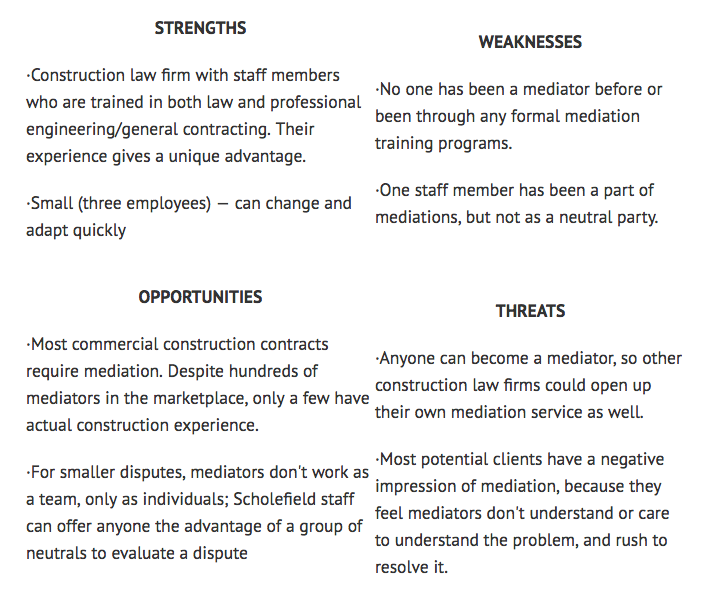
\includegraphics[width=\textwidth]{SWOTExample}
    \caption{Beispiel einer SWOT-Analyse. Quelle: http://www.businessnewsdaily.com/4245-swot-analysis.html}
    \label{fig:SWOTExample}          
\end{figure}

\subsubsection{PEST}
Bei der PEST-Analyse ist das Ziel, die politische, ökonomische, soziokulterelle und technologische Umfeld des Kunden zu verstehen. Dies ist eine reine Umfeld-Analyse und interne Punkte werden nicht aufgelistet. \\
\\
Da in den meisten Fällen bei der Analyse der Kunden für ein CSIRT sowohl interne wie auch externe Faktoren wichtig sind, bietet es sich an eine SWOT- und eine PEST-Analyse zu machen. So kann von Anfang an sichergestellt werden, dass nicht bereits bei der Planung des CSIRT in die falsche Richtung optimiert wird.

\subsection{Festlegen des Aufgabenbereichs}
Als nächstes muss der Aufgabenbereich des CSIRT definiert werden. Dies sollte eine möglichst kurz und knappe Formulierung sein, da diese der Grundstein des CSIRT ist und im besten Fall über Jahre hinweg Gültigkeit hat und nicht angepasst wird. Generell werden diese Formulierungen allgemein gehalten und enthalten keine spezifischen, prozessbedingten Angaben.

\subsection{Ausarbeitung des Geschäftsplans}
Nachdem der Aufgabenbereich definiert wurde, werden spezifischere Angaben im Geschäftsplan gemacht. 

\subsubsection{Finanzierung}
Oft ist in der Praxis die Finanzierung an ein bestimmtes Budget geknüpft. Die wichtigsten Faktoren sind die Dienstzeiten sowie die Anzahl Personenstellen, die für das CSIRT arbeiten.\\
\\
Dem gegenüber steht ein mögliches Ertragsmodell. Hierbei kommt es darauf an, an welche Kundenbedürfnisse sich das CSIRT richtet. Ist das CSIRT z.B. für die öffentliche Hand, sind Subventionen und Gelder vom Staat eine Option. Eine andere Option ist ein Mitgliedermodell mit Zusatzertrag gemäss Aufwand für Zusatzdienste z.B. Sicherheitsaudits.

\subsubsection{Organisation und Einstellen von Mitarbeitern}
Es gibt verschiedene Organisationsmodelle, die für ein CSIRT in Frage kommen. Entweder kann die CSIRT als eigenständige Organisation fungieren (d.h. mit eigener Geschäftsleitung etc.) oder kann als Team innerhalb einer bestehenden Organisation aufgebaut werden. Bei einer verteilten Organisation kann auch in Betracht gezogen werden, aus allen Standorten eine Person zu verpflichten. In der Praxis ist es schwierig, die genau erforderliche Anzahl Mitarbeiter zu bestimmen. Die ENISA spricht von mindestens vier Vollzeitstellen für das Verteilen von Security Advisories und Behandlung von Vorfällen. Übernimmt die CSIRT weitere Verantwortungen und muss z.B. Schichtdienst leisten, spricht die ENISA von mindestens 12 Vollzeitstellen. Hier gilt es die definierten Aufgabengebiete zu analysieren und die Kundenbedürfnisse korrekt zu analysieren. Eine Koordination mit anderen CSIRT kann von Vorteil sein, um z.B. eine 24/7 Abdeckung zu erhalten, bedingt aber das Lösen von anderen logistischen Herausforderungen.

\subsubsection{Richtlinien für die Informationssicherheit}
Je nach Kundentyp differenzieren die zu erstellenden Richtlinien zur Informationssicherheit. Es werden die betrieblichen sowie die administrativen Abläufe und Prozesse definiert. Wichtig dabei ist, dass nationale Richtlinien und Gesetze angewendet und befolgt werden. Viele Länder verfügen z.B. über Datenschutzgesetze, welche von allen eingehalten werden müssen. Ausserdem müssen Richtlinien definiert werden, die z.B. besagen wie Informationen klassifiziert und veröffentlicht werden. Grundsätzlich ist es zu empfehlen Security Advisories öffentlich zugänglich zu machen. Schwachstellen in Kunden-Systemen dürfen z.B. nicht vor dessen Behebung veröffentlicht werden. Eine genaue Spezifikation der Abläufe und Klassifikationen hilft dabei keine Kunden zu verärgern oder Gesetze zu missachten. Hier ist es auch wichtig die Geschäftsleitung mit einzubeziehen, damit organisationsweite Richtlinien mit eingebracht werden können. Natürlich sollte die Geschäftsleitung im gesamten Prozess mindestens ``informiert`` (siehe RASCI~\citep{rasci}) sein. In den meisten Fällen ergibt es jedoch Sinn, die Geschäftsleitung möglichst früh und eng einzubinden.

\section{Betrieb}
Nachfolgend werde ich einige Beispiele von Betriebsfällen nennen und erläutern, was dabei zu beachten ist.

\subsection{Analyse von Klienten}
Um für das Klientel die wichtige Aufgabe eines CSIRT auszuführen, ist es unabdingbar sich von der Umgebung der Klienten ein Bild zu machen. Dabei wird ein genaues Inventar geführt, welche Software bei welchen Kunden im Einsatz ist. Nur so kann effektiv informiert werden, falls eine Sicherheitslücke gefunden wird und entsprechend die Lage beurteilt werden. Wichtig dabei ist, dass diese auch aktuell gehalten wird, da ansonsten Warnungen gesendet werden, welche den Kunden gar nicht mehr betreffen. Dies dient zudem als Grundlage für alle weiteren Fälle.

\subsection{Alarme und Warnungen}
Anhand der oben erstellen Software-Liste können aktuelle und akute Sicherheits- und Bedrohungswarnungen an die Kunden gesendet werden. Hierbei gilt es zu beachten, dass nur Meldungen an Kunden gesendet werden, welche tatsächlich auch von dieser Vulnerability betroffen sind. Ansonsten führt das schnell zu einer ``Geht mich ja nichts an``-Wahrnehmung und die Kunden werden entsensibilisiert, was genau das Gegenteil des Zweckes einer CSIRT ist. Damit der Kunde die Bedrohung entsprechend einschätzen kann, ist es zu bevorziehen jeweils auch eine Analyse der Auswirkung des Incidents zu errechnen. Hierbei bedeutet die Auswirkung die Eintrittswahrscheinlichkeit multipliziert mit dem Risiko. \\
\\
Wichtig ist auch jeweils eine Empfehlung (z.B. Patch einspielen) für jedes Bulletin rauszugeben, damit die Kunden genau wissen, wie sie die Bedrohungslage verringern können. Zusätzlich ist es wichtig, dass diese Nachrichten durch den Kunden als vertrauenswürdig eingestuft werden können. Hierfür kann z.B. E-Mail-Signierung via GPG verwendet werden.

\subsection{Schulungen}
Ein weiterer, sehr wichtiger Punkt sind regelmässige Schulungen. Die IT-Landschaft und dessen Bedrohungen und Gefahren ändern sich fast täglich. Es ist wichtig, dass Angestellte immer auf dem aktuellsten Stand der Informationen sind, damit diese Kunden ihr Wissen entsprechend weitergeben können.\\
\\
Eine Sensibilisierung der Kunden ist genauso wichtig. Wenn ein Kunde zwar die Meldung erhält, dass es eine Bedrohung der IT-Sicherheit gibt, diese aber ignorieren, bzw. entgegen der Empfehlung als ``unwichtig`` einstufen, kann dies zu gravierenden Problemen führen. Daher ist es auch wichtig, Schulungen für Kunden zu veranstalten, um diese zu sensibilisieren.

\nomenclature[z-ENISA]{$ENISA$}{European Union Agency for Network and Information Security}
\nomenclature[z-swot]{$SWOT$}{Strengths, Weaknesses, Opportunities, Threats}
\nomenclature[z-pest]{$PEST$}{Political, Economical, Social, Technological}
\nomenclature[z-gpg]{$GPG$}{GNU Pretty Good Privacy}